\section{Envisioned final product}
A lot to be critical about this design, e.g. it doesn't really account for how braille is read and the convenience of keeping one's fingers in place. It is essentially a braille version of a sighted product.
\begin{figure}
\centering
    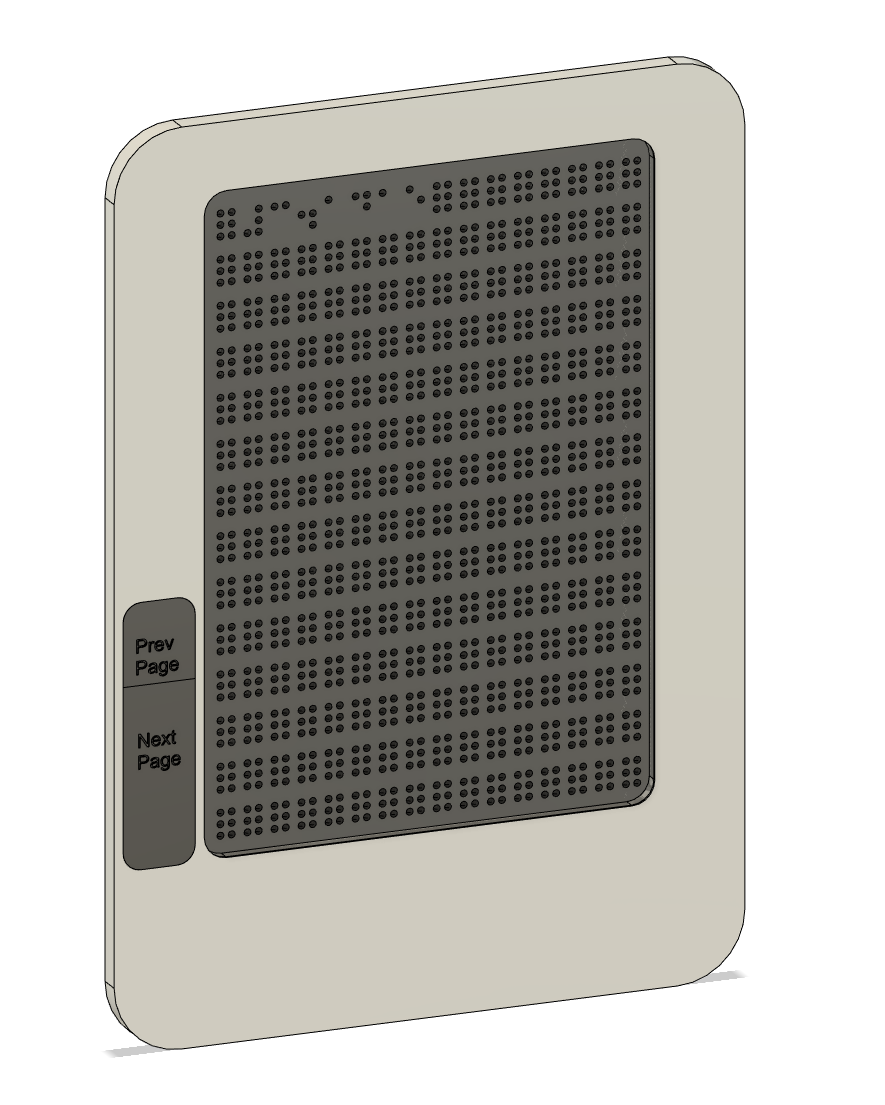
\includegraphics[width=0.4\textwidth]{figures/e-reader.png}
\caption[Envisioned finished product]{Envisioned finished product. A Braille version of a standard e-reader aimed to provide broadened access and display information a traditional Braille device can't.}
\label{fig:e-reader.png}
\end{figure}

% \subsection{Encoding}
% Figure \ref{fig:encoding.png} describes the initial approach to convert text into braille given a device with 16 addressable cells.
% \begin{figure}
% \centering
%     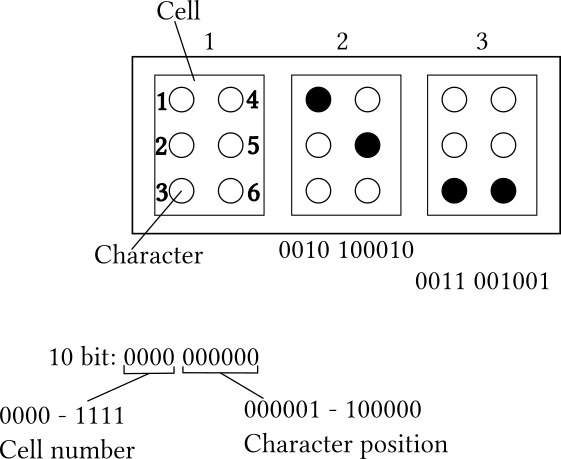
\includegraphics[height=5cm]{figures/encoding.png}
% \caption{Early idea for serial encoding of up to 16 braille cells.}
% \label{fig:encoding.png}
% \end{figure}

\section{Actuator technology}
    \subsection{Addressable cell}
        \subimport{technologies/}{addressable-cell.tex}
    \subsection{Individually addressable characters}
        \subsubsection{Piezoelectric}
        \subimport{technologies/}{piezoelectric.tex}
        
        \subsubsection{Pneumatic}
        \subimport{technologies/}{pneumatic.tex}

        \subsubsection{Magnetic}
        \subimport{technologies/}{magnetic.tex}

        \subsubsection{Others}
        \subimport{technologies/}{others.tex}